\documentclass[10pt,prl,aps,showpacs,twocolumn,unsortedaddress,showkeys,linenumbers]{revtex4-1}
\usepackage{subcaption}
\usepackage{amssymb}
\usepackage{amsmath}
\usepackage{commath}
\usepackage{graphicx,bm}
\usepackage{verbatim}
\usepackage{color}

\captionsetup[subfigure]{labelformat=brace}

%\\\templatetype{pnasresearcharticle} % Choose template 

%\title{Invariances in gain control of olfactory receptor neurons enhances the combinatorial coding fidelity}
%\title{Invariances in gain control of olfactory receptor neurons enhances the fidelity of an odor code}
%\title{Universal front-end gain control aids robust combinatorial odor coding in naturalistic environments}
%\title{Weber-Fechner gain control in olfactory receptor neurons enhances combinatorial coding fidelity}
%\title{Weber-Fechner gain control in olfactory receptor neurons enhances the fidelity of odor coding}
%\title{Weber-Fechner gain control enhances the fidelity of combinatorial odor coding}
\begin{document}


\title{Front-end Weber-Fechner gain control \\ enhances the fidelity of combinatorial odor coding}


% Use letters for affiliations, numbers to show equal authorship (if applicable) and to indicate the corresponding author

% Please include corresponding author, author contribution and author declaration information
%\authorcontributions{N.K. and T.E. conceived the project, analyzed the results, and wrote the manuscript. N.K. performed all calculations. T.E. supervised the project.}
%\authordeclaration{Authors declare no conflict of interest}
%\equalauthors{\textsuperscript{1}A.O.(Author One) and A.T. (Author Two) contributed equally to this work (remove if not applicable).}
%\correspondingauthor{\textsuperscript{2}To whom correspondence should be addressed. E-mail: thierry.emonet@yale.edu}

% Keywords are not mandatory, but authors are strongly encouraged to provide them. If provided, please include two to five keywords, separated by the pipe symbol, e.g:
\keywords{Insect olfaction $|$ Adaptation $|$ Compressed sensing $|$ Olfactory receptor neurons $|$ Combinatorial coding $|$ Orco} 

\begin{abstract}
        In a previous paper (Gorur-Shandilya et al 2017), we showed that \textit{Drosophila} olfactory receptor neurons (ORNs) expressing the co-receptor Orco scale their gain inversely with mean odor intensity, according to the Weber-Fechner law of psychophysics. Here we investigate the implications of this front-end mechanism for odor coding capacity in natural environments, where the intensity and timescales of odor signals can span several orders of magnitude, and odors can mix together. We find that ORN adaptation promotes the reconstruction of odor identity from dynamic odor signals, even in the presence of confounding background odors and rapid intensity fluctuations. These enhancements are further aided by known downstream transformations in the antennal lobe and mushroom body. Our results, which are applicable to various odor classification and reconstruction schemes, stem from the fact that ORN adaptation is not intrinsic to the identity of the receptor involved. {\color {blue} Instead, a feedback mechanism adjusts receptor sensitivity based on the activity of the receptor-Orco complex, in accordance with the Weber-Fechner law. This common scaling of the gain across Orco-expressing ORNs may be one of the features of ORN adaptation that helps preserve combinatorial odor codes in naturalistic landscapes.}
     

     

    
    
    %Instead a feedback mechanism, likely involving the universal co-receptor Orco, adjusts the sensitivity of olfactory receptors via their activity, adjusts receptor sensitivity based on the activity of the olfactory receptor complex, in accordance with the Weber-Fechner law. 
    
    %Hence, the common scaling of the gain with respect to mean odor intensity across Orco-expressing ORNs might be one of the key features of ORN adaptation that enable the maintenance of the combinatorial coding in flying insects.
    
    %Hence, conservation of co-receptor Orco across flying insects might stem in part from its role in enabling a receptor invariant adaptation mechanism for combinatorial coding.  
    
\end{abstract}

%\dates{This manuscript was compiled on \today}
%\doi{\url{www.pnas.org/cgi/doi/10.1073/pnas.XXXXXXXXXX}}

% Added to get write linespread as published articles
%\\\linespread{0.9}

% Set paragraph spacing to zero.
\setlength{\parskip}{0cm plus0mm minus0mm}

\author{Nirag Kadakia}
\affiliation{Department of Molecular, Cellular, and Developmental Biology, Yale University, New Haven, CT 06511}
\author{Thierry Emonet*} 
\affiliation{Department of Molecular, Cellular, and Developmental Biology}
\affiliation{Department of Physics, Yale University, New Haven, CT 06511}
\affiliation{*Corresponding Author}

% Optional adjustment to line up main text (after abstract) of first page with line numbers, when using both lineno and twocolumn options.
% You should only change this length when you've finalised the article contents.
%\verticaladjustment{-2pt}

\maketitle
%\thispagestyle{firststyle}
%\ifthenelse{\boolean{shortarticle}}{\ifthenelse{\boolean{singlecolumn}}{\abscontentformatted}{\abscontent}}{}

%%%%%%%%%%%%%%%%%%%%%%%%%%%%%%%%%%%%%%%%%%%%%%%%%%%%%%%%%%%%%%%%%
%%%%%%%%%%%%    		INTRODUCTION	    		%%%%%%%%%%%%%
%%%%%%%%%%%%%%%%%%%%%%%%%%%%%%%%%%%%%%%%%%%%%%%%%%%%%%%%%%%%%%%%%



Animals identify and discriminate odors using olfactory receptors (Ors) expressed in olfactory receptor neurons (ORNs)~\cite{chemoreceptors_review,buck1991novel,or_discovery_carlson,or_discovery_vosshall}. Individual ORNs, which typically express a single Or, respond to many odorants, while individual odorants activate many distinct ORNs~\cite{friedrich1997combinatorial,hallem_carlson,mosquito_combinatorial_coding,nara2011large}. Odors are  thus encoded by the combinatorial patterns of activity they elicit in the sensing periphery~\cite{malnic1999combinatorial, mosquito_combinatorial_coding, hildebrand1997mechanisms, hallem_carlson, debryune_odor_coding, friedrich1997combinatorial}, patterns  decoded downstream into behavioral response~\cite{early_olfactory_processing, louis_chemotaxis}.  Still, ethologically-relevant odors are often mixed with background ones~\cite{coding_background, odor_backgrounds} and intensity can vary widely and rapidly as odors are carried by the wind~\cite{murlis_odor_plumes, fluid_dynamics_chemosensory, celani, carde_navigation}. How are odors recognized reliably despite these confounds? %Various mechanisms have been suggested. 
In \textit{Drosophila melanogaster}, ORN dose response curves exhibit similar Hill coefficients but distinct power-law distributed activation thresholds~\cite{hallem_carlson, si2017invariances}, which together with inhibitory odorants enhance coding capacity~\cite{si2017invariances, Cao_Tu_WL, hallem_carlson, stevens}. In antennal lobe (AL) glomeruli, mutual lateral inhibition normalizes population response, reducing the dependency of activity patterns on odor concentration~\cite{lateral_inh_asahina, divisive_normalization}. Further downstream, sparse connectivity to the mushroom body (MB) helps maintain neural representations of odors, and facilitates compressed sensing and associative learning schemes~\cite{abbott_axel, litwinkumar, vijay_1, stevens_2}. Finally, temporal features of neural responses contribute to concentration-invariant representations of odor identity~\cite{stopfer_nat_neuro, stopfer_temporal_model, stopfer_temporal_channel, primacy_coding}.

Here we examine how short-time ORN adaptation at the very front-end of the insect olfactory circuit contributes to the fidelity of odor encoding. Our theoretical study is motivated by the recent discovery of invariances in the signal transduction and adaptation dynamics of ORNs expressing the co-receptor Orco. %While for some odor-Or combinations, ORN responses can exhibit large differences, such as super-sustained responses~\cite{montague2011similar} or specialized responses to danger signals~\cite{geosmin}, for many odor-Or combinations the deconvolution of stimulus dynamics from neuron responses produces highly stereotyped filters~\cite{martelli,si2017invariances}. 
ORN response is initiated upon binding of odorant molecules to olfactory receptors (ORs), opening the ion channels they form with the co-receptor Orco~\cite{Orco, orco_structure}. Because of differences in odor-receptor affinities, the responses of ORNs to diverse odorants of the same concentration differ widely~\cite{hallem_carlson,montague2011similar,geosmin}. In contrast, downstream from this input nonlinearity, signal transduction and adaptation dynamics exhibit a surprising degree of invariance with respect to odor-receptor identity: reverse-correlation analysis of ORN response to fluctuating stimuli produces highly stereotyped, concentration-invariant response filters~\cite{martelli,si2017invariances, srinivas_elife}.

These properties stem in part from an apparently invariant adaptive scaling law in ORNs: gain varies inversely with mean odor concentration according to the Weber-Fechner Law of psychophysics~\cite{weber1996eh,fechner2012elemente}, irrespective of the odor-receptor combination~\cite{srinivas_elife,cafaro_WL,cao_WL}. This invariance can be traced back to adaptative feedback mechanisms in odor transduction, upstream of ORN firing~\cite{nagel_wilson_biophysical,cao_WL,cafaro_WL,srinivas_elife}, which depend on the activity of the signaling pathway rather than on the identity of its receptor~\cite{nagel_wilson_biophysical}. 
The generality of the adaptive scaling suggests it could be mediated by the highly conserved Orco co-receptor~\cite{orco_structure,getahun2013insect,getahun2016intracellular,Guo_Smith}. Indeed, phosphorylation sites have been recently identified on Orco, some being implicated in odor desensitization, albeit over much longer timescales~\cite{Guo_Smith_review,Guo_Smith}. 


\begin{figure*}[!tb]
	\centering
	\begin{subfigure}[t]{\linewidth}
		\phantomsubcaption
		\label{fig:tuning_curves_a}
	\end{subfigure}
	\begin{subfigure}[t]{0\linewidth}
		\phantomsubcaption
		\label{fig:tuning_curves_b}
	\end{subfigure}
	\begin{subfigure}[t]{0\linewidth}
		\phantomsubcaption
		\label{fig:tuning_curves_c}
	\end{subfigure}
	\begin{subfigure}[t]{0\linewidth}
		\phantomsubcaption
		\label{fig:tuning_curves_d}
	\end{subfigure}
	\begin{subfigure}[t]{0\linewidth}
		\phantomsubcaption
		\label{fig:tuning_curves_e}
	\end{subfigure}
	\begin{subfigure}[t]{0\linewidth}
		\phantomsubcaption
		\label{fig:tuning_curves_f}
	\end{subfigure}
	\begin{subfigure}[t]{0\linewidth}
		\phantomsubcaption
		\label{fig:tuning_curves_g}
	\end{subfigure}
	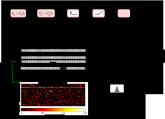
\includegraphics[width=\linewidth]{figures/1_tuning_curves}
	\caption{\footnotesize{
		\textbf{Simple ORN model.}~\cite{srinivas_elife} \textbf{A}~Or/Orco complexes of type $a$ switch between active $\textup{C}^*_a$ and inactive conformations $\textup{C}_a$. Binding an exitatory odorant ($\textup{S}$ in the diagram) favors the active state. The active fraction is determined by the free energy difference between inactive and active conformations of the Or/Orco complex in its unbound state, $\epsilon_a(t)$ (in units of $k_B T$), and by odorant binding with affinity constants $\mathbf{K}^*_a=(K^*_{a1},...,K^*_{ai},...,K^*_{aN})$ and $\mathbf{K}_a$ for the active and inactive conformations, respectively (Eqs.~\ref{eq:steady_state_gen_ex}-\ref{eq:steady_state_act_OR}). Adaptation is mediated by a negative feedback~\cite{nagel_wilson_biophysical} from the activity of the channel onto the free energy difference $\epsilon_a(t)$ with timescale $\tau$. ORN firing rates $r_a(t)$ are generated by passing $A_a(t)$ through a linear temporal filter $h(t)$ and a nonlinear thresholding function $f$.
		\textbf{B}~Odors are represented by $N$-dimensional vectors $\mathbf{s}=(s_1,...,s_i,...,s_N)$ , whose components $s_i$ are the concentrations of  the individual molecular constituents  of $\mathbf s$. 
		%\textbf{C}~Active binding constants are distributed as a power-law with coefficient $\alpha=0.35$~\cite{si2017invariances}.
		\textbf{C}~Step-stimulus firing rate of 50 ORNs to the $N$=150 possible monomolecular odorants $\mathbf s = s_i$, given  power-law distributed afffinity constants~\cite{si2017invariances}.
		\textbf{D}~Temporal responses of a representative ORNs to a pulse stimulus, for a single odorant at several intensities (left), or to many odorants of the same intensity (right).
		\textbf{E}~Representative ORN tuning curves (a single row of the response matrix in C, ordered by magnitude). Tuning curves are diverse, mimicking measured responses~\cite{hallem_carlson}.
		{\color {blue} 
		\textbf{F}~Dose-response of an ORN before (black) and after adaptation to either a low (yellow) or high (magenta) odor concentration.  
		\textbf{G} Same, but the ORN was allowed to first adapt to one of various backgrounds of differing identities, before the foreground (same as in F) was presented. Also shown is the specific case when the foreground and background have the same identity (dashed lines).}}
		}
		\label{fig:tuning_curves}
\end{figure*}

While in a simpler system such as \textit{E. coli} chemotaxis~\cite{EmonetReview}, adaptive feedback via the Weber-Fechner Law robustly maintains sensitivity over concentration changes, the implication for a multiple-channel system -- which combines information from hundreds of cells with overlapping receptive fields  -- is less clear. Here we combine a biophysical model of ORN adaptive response and neural firing with various sparse signal decoding frameworks to explore how ORN adaptation with Weber-Fechner scaling affects combinatorial coding and decoding of odor signals spanning varying degrees of intensity, molecular complexity, and temporal structure. We find that this front-end adaptive mechanism promotes the accurate discrimination of odor signals from backgrounds of varying molecular complexity, and aids other known mechanisms of neural processing in the olfactory circuit to maintain representations of odor identity across environmental changes. %both in static odor environments  and in fluctuating ones.
%We also investigate our framework in the context of the primacy coding hypothesis  -- that odors are encoded entirely by the few earliest responding ORNs~\cite{primacy_coding, primacy_math}, finding that primacy coding is both consistent with and enhanced by front-end adaptation. 


\section*{Results}



%%%%%%%%%%%%%%%%%%%%%%%%%%%%%%%%%%%%%%%%%%%%%%%%%%%%%%%%%%%%%%%%%
%%%%%%%%%%%%    		MODEL DESCRIPTION    		%%%%%%%%%%%%%
%%%%%%%%%%%%%%%%%%%%%%%%%%%%%%%%%%%%%%%%%%%%%%%%%%%%%%%%%%%%%%%%%



\subsection*{Model of ORN sensing repertoire}

To model ORN firing rates in response to time-dependent odor signals, we extended a minimal model~\cite{srinivas_elife} that reproduces the Weber-Fechner gain adaptation and firing rate dynamics measured in individual \textit{Drosophila} ORNs in response to Gaussian and naturalistic signals (code available on GitHub\cite{code}). 

We consider a repertoire of $M=50$ ORN types that each express one type of Or together with the co-receptor Orco~\cite{Orco}. Within ORNs of type $a=1,...,M$, Or-Orco complexes form non-selective cation channels~\cite{orco_structure} (Fig.~\ref{fig:tuning_curves_a}) that switch between active and inactive conformations, while simultaneously binding to odorants $i$ with affinity constants, $K^*_{ai}$ and $K_{ai}$, respectively~\cite{nagel_wilson_biophysical,srinivas_elife}. For simplicity we only consider agonists, i.e. $K^*_{ai} > K_{ai}$, and assume receptors can only bind one odorant at a time. The analysis can easily be extended to include inhibitory odorants, which increases coding capacity~\cite{Cao_Tu_WL}. Dissociation (inverse affinity) constants are chosen from a power law distribution ($\alpha = 0.35$) recently found across ORN-odor pairs in \textit{Drosophila} larvae~\cite{si2017invariances}. For a handful of ORNs, we choose a very large value for one of the $K^*_{ai}$ to mimic high responders to private odorants relevant to innate responses~\cite{geosmin}. These private odors do not affect the general findings. 

Assuming that odorant binding and conformation changes are faster than other reactions in the signaling pathway, the fraction of channels of type $a$ that are active at steady state is:

{\color {blue} 
\begin{align}
A_a(t) &= \frac{\textup{C}_a^* + \textup{C}_a^* \mathbf{K}^*_a\cdot\mathbf{s}(t)}{\textup{C}_a^* +\textup{C}_a^* \mathbf{K}^*_a\cdot\mathbf{s}(t) + \textup{C}_a +\textup{C}_a \mathbf{K}_a\cdot\mathbf{s}(t) }. 
%\nonumber \\
%&= 1/\left(1 + \frac{C_a + \sum_i C_a s_i}{C_a^* + \sum_i C^*_a s_i}\right)
\label{eq:steady_state_gen_ex}
\end{align}

$\textup{C}_a$ and $\textup{C}_a^*$ represent unbound channels in the inactive and active conformation. Here, $\mathbf{K}_a\cdot\mathbf{s}(t)=\sum_i^N K_{ai} s_i(t)$, where $s_i(t)$ is the time-dependent concentration of the $i$-th monomolecular component of the odor signal ${\bf s}(t)$ at time $t$ (Fig.~\ref{fig:tuning_curves_b}).  $N=150$ is the size of the molecular odorant space (Fig.~\ref{fig:tuning_curves_b}).
%Enforcing detailed balance on the 4-state cycle containing odorant $s_i$ (Fig.!!), we can express the free energy of activation when bound in terms of the free energy of activation when unbound and the disassociation constants: $\epsilon_{ai} = \epsilon_a + \ln(K^*_{ai}/K_{ai})$. For excitatory odorants, $K^*_{ai} < K_{ai}$, which implies that $\epsilon_{ai} < \epsilon_a$; intuitively, receptors are more likely to be active (and the ORN to be firing) when bound. 
Eq.~\ref{eq:steady_state_gen_ex} can be rearranged as (derivation in Methods):

\begin{align}
A_a(t) &= \left[1 + \exp\left(\epsilon_a(t) + \ln\left(\frac{1 + \mathbf{K}_a\cdot\mathbf{s}(t)}{1 + \mathbf{K}^*_a\cdot\mathbf{s}(t)}\right)\right)\right]^{-1}. 
%A_a(t) &= \left[1 + e^{\ln\left(\frac{1 + \sum_i^N %s_i(t)/K_{ai}}{1 + \sum_i^N %s_i(t)/K^*_{ai}}\right)+\epsilon_a(t)}\right]^{-1}. %\nonumber \\
%A_a(t) &= \frac{1}{1 + e^{E_a(t)}} \nonumber \\
%E_a(t) &= \epsilon_a(t) + \ln\left[\frac{1 + \sum_i^N s_i(t)/K_{ai}}{1 + \sum_i^N s_i(t)/K^*_{ai}}\right],
\label{eq:steady_state_act_OR}
\end{align}

The two terms in the exponential represent the change in the channel's free energy due to the binding of odorant $i$, and the free energy difference %$\epsilon_a(t)=\ln{\left(C_a/C^*_a\right)}$ 
$\epsilon_a$ between the unbound states $\textup{C}_a$ and $\textup{C}_a^*$, %inactive and active conformations of unbound receptors
in units of $k_B T$. Because $K^*_{ai} > K_{ai}$, a sudden increase in the concentration of excitatory odor results in an % decrease in $E_a$ and corresponding 
increase in activity $A_a$.

Upon prolonged stimulation, ORNs adapt. At least one form of adaptation, which takes place over short time scale, $\tau\simeq 250$ ms~\cite{srinivas_elife}, involves a negative feedback of the Or-Orco channel activity onto the channel sensitivity~\cite{nagel_wilson_biophysical,srinivas_elife}. To model this adaptation process, we assume that inward currents elicited by activating Or-Orco channels eventually result in an increase of the free energy difference $\epsilon_a(t)$, possibly via a feedback onto Orco~\cite{orco_structure}:

\begin{align}
\tau\frac{d\epsilon_a(t)}{dt} = {A}_{a}(t) - A_{0a},
\label{eq:adaptation_dynamics}
\end{align}

where $\epsilon_{\textup{L}, a} < \epsilon_a(t) < \epsilon_{\textup{H}, a}$. The lower bound $\epsilon_{\textup{L}, a}$ determines the spontaneous activity of the channel. The higher bound $\epsilon_{\textup{H}, a}$ determines the concentrations of odors at which adaptation is unable to keep up and saturation occurs~\cite{srinivas_elife}. Through these dynamics, $\epsilon_a(t)$ can compensate for changes in free energy due to ligand binding (see Eq.~\ref{eq:steady_state_act_OR}), returning the activity $A_a$ towards an adapted level $A_{0a}$ above the spontaneous activity. Since $\epsilon_a$ is bounded below, a minimum amount of signal intensity is needed for adaptation to kick in. 
}
Finally, the firing rate is modeled by passing the activity $A_a(t)$ through the derivative-taking bi-lobed filter $h(t)$ and a rectifying nonlinearity
$f$~\cite{srinivas_elife}:

\begin{align}
r_a(t)=f\left(h(t) \otimes A_a(t)\right),
\label{eq:firing_machinery}
\end{align}

where $\otimes$ is convolution. When deconvolved from stimulus dynamics, the shapes of the temporal kernels of \textit{Drosophila} ORNs that express Orco tend to be stereotyped for many odor-receptor combination~\cite{martelli,srinivas_elife,si2017invariances} 
{\color {blue} 
(although there are known exceptions such as super-sustained responses~\cite{montague2011similar}).
}
Moreover, adaptation is not intrinsic to the receptor~\cite{nagel_wilson_biophysical}. Accordingly, for simplicity $\tau$, $h(t)$, and $f$ are assumed independent of receptor and odorant identities.

This minimal model reproduces the essential features of ORN response to odorant pulses~\cite{nagel_wilson_biophysical, martelli, cao_WL}. 
{\color {blue} 
In the absence of stimulus, ORNs fire spontaneously at rates (1-10 Hz)~\cite{hallem_carlson} set by the lower free energy bound $\epsilon_{\textup{L}, a}$, which we choose from a normal distribution (Fig.~\ref{fig:tuning_curves_d})~\cite{nagel_wilson_biophysical, martelli}. For sufficiently strong stimuli, adaptation causes $\epsilon_a$ to increase, compensating for the drop in free energy difference due to ligand binding. This gradually reduces the firing rate to a steady state level $r(A_{0a}) \simeq$ 30-40 Hz~\cite{srinivas_elife}  (Fig.~\ref{fig:tuning_curves_d}). The diversity of temporal firing responses and tuning curves measured experimentally ~\cite{hallem_carlson,montague2011similar, stopfer_nat_neuro, stopfer_temporal_channel,stopfer_temporal_model} arise naturally in the model due to the distribution of chemical affinity constants and the nonlinearity of Eq.~\ref{eq:steady_state_act_OR} (Figs.~\ref{fig:tuning_curves_b}-\ref{fig:tuning_curves_e}). 

The model also reproduces Weber-Fechner scaling of the gain with the inverse of the mean odorant intensity $\bar{s}_i$~\cite{srinivas_elife, cao_WL}. For small fluctuations $\Delta s_i$ around $\bar{s}_i$, we have from Eq.~\ref{eq:steady_state_act_OR} that $\Delta A_a/\Delta s_i\simeq A_a\left(\bar{s}_i\right)\left(1-A_a\left(\bar{s}_i\right)\right)/\bar{s}_i$, whereby Weber's Law is satisfied provided $A_a(\bar{s}_i)$ is approximately constant (derivation in Methods). In our model, since the rate of adaptation depends only on the activity of the ion channel (right hand-side of Eq.~\ref{eq:adaptation_dynamics}), then in the adapted state we have $A_a\left(\bar{s}_i\right)\simeq A_{0a}$, ensuring that the gain scales like $1/\bar{s}_i$. This process adjusts the sensitivity of the ORN by matching the dose responses to the mean signal concentration, while maintaining their log-slopes (Fig.~\ref{fig:tuning_curves_f}). However, for foreground odors mixed with background odors to which the system has adapted, the dose response curves now exhibit background-dependent shifts (Fig.~\ref{fig:tuning_curves_g}). %Still, though shifted, these curves maintain their log-slopes as a consequence of Weber-Fechner scaling. Below, we will see that, despite these shifts, the maintenance of this scaling plays a critical role in preserving combinatorial odor codes (Fig.~\ref{fig:tuning_curves_g}). 
}

While this phenomenological model could be extended to include further details -- e.g. we could relax the quasi-steady-state assumption in Eq.~\ref{eq:steady_state_act_OR} and use a more complex model for channel adaptation and neural firing~\cite{srinivas_elife} -- this minimally-parameterized form captures the key dynamical properties of Orco-expressing ORNs relevant to our study: receptor-independent adaptation~\cite{nagel_wilson_biophysical} with Weber-Fechner scaling~\cite{srinivas_elife, cafaro_WL,cao_WL} that maintains response time independent of mean stimulus intensity~\cite{martelli,srinivas_elife}, along with a diversity of temporal firing patterns in response to a panel of monomolecular odorants~\cite{hallem_carlson, montague2011similar, stopfer_nat_neuro, stopfer_temporal_channel, stopfer_temporal_model} (Fig.~\ref{fig:tuning_curves_d}-\ref{fig:tuning_curves_e}).


 



%%%%%%%%%%%%%%%%%%%%%%%%%%%%%%%%%%%%%%%%%%%%%%%%%%%%%%%%%%%%%%%%%
%%%%%%%%%%%%		CODING CAPACITY SECTION			%%%%%%%%%%%%%
%%%%%%%%%%%%%%%%%%%%%%%%%%%%%%%%%%%%%%%%%%%%%%%%%%%%%%%%%%%%%%%%%




\subsection*{Front-end Weber-Fechner adaptation preserves odor coding among background and intensity confounds.}

\begin{figure*}[!htb]
	\centering
	\begin{subfigure}[t]{\linewidth}
		\includegraphics[width=\textwidth]{figures/2_coding_representation}
		\phantomsubcaption
		\label{fig:coding_a}
	\end{subfigure}
	\begin{subfigure}[t]{0\linewidth}
		\phantomsubcaption
		\label{fig:coding_b}
	\end{subfigure}
	\begin{subfigure}[t]{0\linewidth}
		\phantomsubcaption
		\label{fig:coding_c}
	\end{subfigure}
	\begin{subfigure}[t]{0\linewidth}
		\phantomsubcaption
		\label{fig:coding_d}
	\end{subfigure}
	\begin{subfigure}[t]{0\linewidth}
		\phantomsubcaption
		\label{fig:coding_e}
	\end{subfigure}
	\caption{\footnotesize{\textbf{Front-end adaptation maintains representations of odor identity across background and intensity confounds.}
	\textbf{A}~Example t-SNE projection of the 50-dimensional vector of ORN firing rates to 2 dimensions. Each point represents the firing response to a distinct odor. Nearby points exhibit similarities in corresponding firing rates.
	\textbf{B}~t-SNE projection of ORN firing rates, where each point represents the response to foreground odor $\mathbf{s}$ (point color) on top of a background odor $\bar{\mathbf{s}}$ (point size). In the adaptive system, $\epsilon_a$ are set to their steady state values given the background odor $\bar{\mathbf{s}}$ alone according to Eq.~\ref{eq:beta} with $\beta=0$. We assumed $A_{0a}=A_0$ for all $a$ (we obtain similar results when $A_{0a}$ are randomly distributed; Fig.~\ref{fig:SI_coding}). Clustering by color implies that responses cluster by foreground odor identity.
    \textbf{C}~Similar to $\mathbf{B}$, but now for odors whose concentrations span 4 decades (represented by point size). Here, the background odor identity is the same for all concentrations. 
    {\color {blue} 
    \textbf{D}~Performance of odor coding as a function of $\beta$, the magnitude of the deviation from Weber-Fechner's law ($\beta=0$: Weber-Fechner's scaling; $\beta=1$: no adaptation; see Eq.~\ref{eq:beta}). Performance is quantified by the silhouette score $H$, which quantifies the degree by which responses cluster by foreground identity versus background identity in the t-SNE projections (1: highly clustered by foreground identity; 0 or slightly negative: not clustered) (\cite{silhouette_score} and Methods). Line: same scaling $\beta_a=\beta$ for all ORNs. Dashed: $\beta_a$ is uniformly distributed between 0 and $2\beta < 1$ (i.e. has mean $\beta$).
    \textbf{E}~Distribution of ORN responses and t-SNE projections for $\beta = 0, 0.13, 0.28, 0.35$ in $\mathbf{D}$. }}
    }
	\label{fig:coding}
\end{figure*}

{\color {blue} 
To investigate how front-end adaptation and its scaling according to Weber-Fechner's law affect the representations of odor identity within the repertoire of ORN response, we quantified the similarity between the responses $\mathbf r_1$ and $\mathbf r_2$ of the ORN repertoire to different simuli $\mathbf{s}_1$ and $\mathbf{s}_2$ by measuring the Euclidean distance between $\mathbf r_1$ and $\mathbf r_2$. Since it is not possible to visualize these 50-dimensional vectors, we projected them onto a lower-dimensional space using t-distributed stochastic neighbor embedding (t-SNE)~\cite{tsne}. Like principle component analysis (PCA), t-SNE preserves similarity between objects (Fig.~\ref{fig:coding_a}), but is more suitable than PCA for objects that are related nonlinearly -- in our case, the dependency of firing rates on odor concentrations (Eq.~\ref{eq:steady_state_act_OR}).
}


We first examined how an adaptive or non-adaptive ORN repertoire encodes odor identity in an odor environment that contains a foreground odor $\mathbf{s}$ atop a background odor $\bar{\mathbf{s}}$ (Fig.~\ref{fig:coding_b}). Both odors are sparse mixtures, with $K \ll N$ odorants of similar concentrations, odor ``identity'' being the particular set of odorants in the mixture. In the adaptive case, we assume that the system has fully adapted to the background $\bar{\mathbf{s}}$ before the foreground $\mathbf{s}$ is presented. This is enacted by calculating the firing response to the foreground odor $\mathbf{r}(\mathbf{s})$ only after having set the $\epsilon_a$ in Eq.~\ref{eq:steady_state_act_OR} to their steady state values in response to the background odor $\bar{\mathbf{s}}$: 
{\color {blue} 
\begin{align}
    \epsilon_{a}(\bar{\mathbf s}) = \ln\left[\frac{1-A_{0a}}{A_{0a}}\right] - \left(1-\beta_a\right)\ln\left(\frac{1 + \mathbf{K}_a\cdot\bar{\mathbf{s}}}{1 + \mathbf{K}^*_a\cdot\bar{\mathbf{s}}}\right),
    \label{eq:beta}
\end{align}

where we have introduced the new parameter $\beta_a$ to allow us to control the scaling of gain adaptation: for $\beta_a=0$ the system exactly follows Weber-Fechner's law, while for $\beta_a=1$ there is no adaptation. For small but nonzero $\beta_a$, the inverse gain scales sub-linearly (see Methods), and the adapted activity $A_a(\bar{\mathbf s})$ increases weakly with background $\bar{\mathbf s}$. In experiments, small deviations from the strict Weber-Fechner scaling on the order of $\beta\simeq 0.1$ are observed (see extended figures in~\cite{srinivas_elife}).
}


With Weber-Fechner's law in place for all ORNs ($\beta_a=0$) responses cluster by the identity of foreground odor, showing that the repertoire of ORNs appropriately encodes the identity of novel odors irrespective of background signals -- once these backgrounds have been ``adapted away'' (Fig.~\ref{fig:coding_b}). 
{\color {blue} 
This is the case regardless of whether $A_{0a}$ is identical or different across neurons (Fig.~\ref{fig:SI_coding}). 
}
In contrast, when the system is non-adaptive, ($\beta_a=1$), the responses exhibit weaker separations by odor identity (Fig.~\ref{fig:coding_b}). Similarly, responses across different odor intensities are well separated by odor identity in the adaptive system, but less so in the non-adaptive system (Fig.~\ref{fig:coding_c}). Calculating the mutual information between odor and ORN response in time shows that the adaptive system retains coding capacity as it confronts novel odors (Fig.~\ref{fig:SI_MI}) whereas the non-adaptive system maintains coding capacity in a far more limited range of odor concentration.


{\color {blue} 
To what extent do the benefits of front-end adaptation for odor coding depend on the precise Weber-Fechner scaling? We repeated the analysis from Fig.~\ref{fig:coding_b} for increasing values of $\beta_a=\beta$ between zero (Weber's law) (perfect adaptation) and one (no adaptation). To generalize Fig.~\ref{fig:coding_b}, we now let the intensities range over two decades.  As $\beta$ increases, the capacity of the system to cluster responses by odor identity degrades (Fig.~\ref{fig:coding_d}). Introducing diversity among ORNs by distributing $\beta_a$'s uniformly between 0 and $2\beta$ (so that the mean is $\beta$) slightly increases performance at high $\beta$ but reduces it at low $\beta$ (Fig.~\ref{fig:coding_d}). Overall, performance of odor coding degrades with $\beta$, as poorly-adapting ORNs begin to saturate (Fig.~\ref{fig:coding_e}). 

Interestingly, besides this general trend, we find that for $\beta$ very close to zero, a small deviation from Weber-Fechner's law instead \textit{improves} odor coding. This arises because of the nonlinearity in the onset of adaptation: adaptation kicks in only when the strength of stimulus is sufficient for the response $A_a$ to exceed $A_{0a}$, so that the right hand-side of Eq.~\ref{eq:adaptation_dynamics} is positive. The minimum background intensity $\bar{s}$ required for this to happen is given by $\epsilon_{\textup{L}, a}=\epsilon_a(\bar{s})$, which, according to equation Eq.~\ref{eq:beta}, increases with $\beta$. This initial effect increases odor coding performance, as the firing rates can distribute more broadly across the dynamical range of the ORNs, before adaptation is effected (Fig.~\ref{fig:coding_e}). 


Thus, while Weber-Fechner's Law scaling largely preserves the representation of foreground odor identity amid backgrounds, in some cases it may benefit from a slight relaxation so that the full dynamical range of the ORNs can be exploited.
}


%%%%%%%%%%%%%%%%%%%%%%%%%%%%%%%%%%%%%%%%%%%%%%%%%%%%%%%%%%%%%%%%%
%%%%%%%%%%%%    		SIGNAL DECODING      	     %%%%%%%%%%%%
%%%%%%%%%%%%%%%%%%%%%%%%%%%%%%%%%%%%%%%%%%%%%%%%%%%%%%%%%%%%%%%%%




\begin{figure*}[t]
	\centering
	\begin{subfigure}[t]{17.7cm}
		\includegraphics[width=17.7cm]{figures/3_decoding_temporal}
		\phantomsubcaption
		\label{fig:decoding_a}
	\end{subfigure}
	\begin{subfigure}[t]{0\linewidth}
		\phantomsubcaption
		\label{fig:decoding_b}
	\end{subfigure}
	\begin{subfigure}[t]{0\linewidth}
		\phantomsubcaption
		\label{fig:decoding_c}
	\end{subfigure}
	\begin{subfigure}[t]{0\linewidth}
		\phantomsubcaption
		\label{fig:decoding_d}
	\end{subfigure}
	\begin{subfigure}[t]{0\linewidth}
		\phantomsubcaption
		\label{fig:decoding_e}
	\end{subfigure}
	\caption{\footnotesize{\textbf{Front-end adaptation promotes accurate odor decoding in static and naturalistic odor environments.}
    \textbf{A}~Odor stimuli produce ORN responses via odor-binding and activation and firing machinery, as described by Eqs.~\ref{eq:steady_state_act_OR}-\ref{eq:firing_machinery}. Odors are then decoded using compressed sensing optimization.  Odors are assumed sparse, with $K$ nonzero components, $K \ll N$. 
    \textbf{B}~Decoding accuracy of foreground odors in the presence of background odors, for a system without Weber Law adaptation. 
    \textbf{C}~Same as $\mathbf {B}$, with Weber Law adaptation.
    \textbf{D}~Recorded trace of naturalistic odor signal; whiffs (signal $> 4$ a.u.) demarcated by purple bars. This signal is added to static backgrounds of different intensities and complexities.
    \textbf{E}~Individual plots show the percent of accurately decoded odor whiffs as a function of background odor intensity, for the non-adaptive (blue) and adaptive (red) systems, for different $\tau_{\textup M}$ (line shades). 
    }}
	\label{fig:decoding}
\end{figure*}


\subsection*{Front-end adaptation enhances odor decoding in complex environments}

{\color {blue} 
How well does the preservation of odor coding  translate to better signal reconstruction from ORNs responses?
%Next, we ask how the universal adaptive feedback might contribute to accurate signal reconstruction from ORN responses. 
One potentially complicating factor is the disparity between sensor dimension and stimulus dimension: while \textit{Drosophila} only express $\sim 60$ Or genes~\cite{olfactory_sensory_map}, the space of odorants is far greater~\cite{vijay_1}. An $N$-dimensional odor signal would naively need $N$ sensory neurons to decode it -- one for each odorant. However, naturally-occurring odors are sparse, typically comprised of only a few odorants. Enforcing sparsity of the signal during decoding greatly restricts the number of possible odors consistent with a given ORN response, suggesting that such high-dimensional signals might be inferred from less than $N$ ORNs. Indeed, the decoding of sufficiently sparse signals from lower-dimensional responses is rigorously guaranteed by the theory of compressed sensing (CS)~\cite{CS_donoho, CS_tao}.} It is unknown whether CS is implemented in the \textit{Drosophila} olfactory circuit~\cite{chlovskii_pevlavan}. Here we use this framework mainly as a tool to quantify how front-end adaptation potentially affects odor decoding, later verifying our conclusions with other classification techniques that incorporate the known architecture of the olfactory system. 

{\color {blue} 
In practice, CS is performed as a constrained linear optimization over the components of the signal vector -- here, the odorant concentrations $s_i$. The constraints in the optimization are $\mathbf r = \mathbf D \mathbf s$, where $\mathbf D$ is a matrix and $\mathbf D$ are the measurements -- here, $\mathbf r$ would be the vector of ORN responses. The cost function to be minimized, $C = \sum_i |s_i|$, enforces sparsity by driving the estimate of each odorant component to zero; the constraints balance this tendency by simultaneously enforcing information from the ORN firing rates. The result is a reconstructed odor signal $\hat {\mathbf s}$ that is as sparse as possible, consistent with the ORN responses $\mathbf{r}$. }

To incorporate the linear framework of CS into our nonlinear odor encoding model, we treat the nonlinear odor encoding exactly, but approximate the decoding to first order around the background concentration. Specifically, we use Eqs.~\ref{eq:steady_state_act_OR}-\ref{eq:firing_machinery} to generate ORN responses $\mathbf r$ for sparse odors $\mathbf s$ having $K \ll N$ nonzero components $s_i = \bar{s}_i + \Delta s_i$, where the mean concentration is $\bar{s}_i$. To reconstruct these signals using CS, we minimize $\sum_i |\Delta s_i|$ while enforcing the constraints $\mathbf r = \mathbf D \Delta \mathbf s$, where $\mathbf D$ is the linearization of Eq.~\ref{eq:steady_state_act_OR} around $\bar{s}_i$ (details in Methods). This linearization simplifies the CS decoding -- namely it enforces a single, global minimum  -- but it is not critical for our general results; see Methods and Fig.~\ref{fig:SI_IHT_est}. The matrix $\mathbf D$ depends on $\epsilon_a$, and as above, we assume precise adaptation by setting $\epsilon_a$ to their steady state values in response to the background odor alone (via Eq.~\ref{eq:beta} with $\beta=0$). In the nonadaptive case, $\epsilon_a$ are held at their minimum values $\epsilon_{\textup L, a}$. 

We first examine how foreground odors are recognized when mixed with background odors of a distinct identity but similar intensities, quantifying decoding accuracy as the percentage of odors correctly decoded within some tolerance (see Methods). Without adaptation, accuracy is maintained within the range of receptor sensitivity for monomolecular backgrounds, but is virtually eliminated as background complexity rises (Fig.~\ref{fig:decoding_b}). The range of sensitivity is broader in the adaptive system, and is substantially more robust across odor concentration and complexity (Fig.~\ref{fig:decoding_c}). 

In realistic odor environments, the concentration and duration of individual odor whiffs vary widely~\cite{celani}. We wondered how well a front-end adaptation mechanism with a single timescale $\tau$ could promote odor identity detection in such environments. As inputs to our coding/decoding framework, we apply a naturalistic stimulus intensity recorded using a photo-ionization detector~\cite{srinivas_elife} (Fig.~\ref{fig:decoding_c}) to which we randomly assign sparse identities from the $N$-dimensional odorant space. To mimic background confounds, we combine these signals with static odor backgrounds, and then calculate the percentage of decoded whiffs. We assume the decoder has short-term memory: detected odor signals are only retained for $\tau_{\textup {M}}$ seconds in the immediate past, {\color {blue} 
bounding the amount of past information utilized in signal reconstruction. 
}

Without ORN adaptation, sufficiently strong backgrounds eliminate the ability to reconstruct the identity of individual odor whiffs, irrespective of the complexity of either the foreground or background odor (Fig.~\ref{fig:decoding_d}, blue lines). In the adaptive system, this is substantially mitigated (red lines in Fig.~\ref{fig:decoding_d}), provided the memory duration $\tau_{\textup {M}}$ is at least as long as the adaptation timescale $\tau$ (darker red lines). Because this short-term adaptation depends on the activity of the Or-Orco channel rather than on the identity of the receptor~\cite{nagel_wilson_biophysical,martelli,srinivas_elife}, the values of $\tau$ and $A_{0}$ were assumed the same for all ORNs; still, our results hold if these invariances are relaxed (Fig.~\ref{fig:SI_broad_tA}-Fig.~\ref{fig:SI_broad_A0}). 
%Thus, we find that universal front-end adaptation with a single timescale promotes detection of naturalistic odor signals amidst confounding backgrounds of varying complexity and intensity.





\subsection*{Front-end adaptation enhances primacy coding}

The primacy coding hypothesis has recently emerged as an intriguing framework for combinatorial odor coding. Here, odor identity is encoded by the set (but not temporal order) of the $p$ earliest responding glomeruli/ORN types, known as primacy set of order $p$~\cite{primacy_coding}. If the activation order of ORNs were invariant to the strength of an odor step or pulse, primacy sets would in principle form concentration-invariant representation of odor identity. Though our coding framework uses the full ORN ensemble in signal reconstruction, some of these responses may contain redundant information, and a smaller primacy subset may suffice. To examine this, we apply our model to a sigmoidal stimulus that rises to half-max in 50 ms, calculating decoding accuracy in time. Since ORNs activate sequentially, the primacy set is defined by the ORN subset active when the odor is decoded. For simple odors, a limited set of earliest responding neurons fully accounts for the odor identity (Fig.~\ref{fig:primacy_coding_a}), in agreement with primacy coding. As expected for more complex odor mixtures, the full repertoire is required for accurate decoding. Primacy coding also predicts that for stronger stimuli, responses occur earlier, since the primacy set is realized quicker, which our framework replicates (Fig.~\ref{fig:SI_primacy}).

Beyond mere consistency, however, front-end adaptation might also enhance primacy coding in different environments, such as background odors, which could scramble primacy sets. To investigate this, we considered again a sigmoidal odor step (odor A), now atop a static background (odor B) to which the system has adapted. We compared the primacy sets of odor A for 1000 different choices of odor B, finding that primacy sets are highly consistent across background confounds for all but the smallest primacy orders (Fig.~\ref{fig:primacy_coding_b}-\ref{fig:primacy_coding_c}). This also holds true for backgrounds of different concentrations (Fig.~\ref{fig:SI_primacy}), suggesting a central role for front-end adaptation in reinforcing primacy codes across differing environmental conditions. 


\subsection*{Contribution of front-end adaptation for odor recognition within the \textit{Drosophila} olfactory circuit}


\begin{figure}[tb]
	\begin{subfigure}[t]{\linewidth}
		\includegraphics[width=\textwidth]{figures/4_primacy_coding}
		\phantomsubcaption
		\label{fig:primacy_coding_a}	
	\end{subfigure}
	\begin{subfigure}[t]{0\linewidth}
		\phantomsubcaption
		\label{fig:primacy_coding_b}
	\end{subfigure}
	\begin{subfigure}[t]{0\linewidth}
		\phantomsubcaption
		\label{fig:primacy_coding_c}
	\end{subfigure}
	\caption{\footnotesize{\textbf{Effect of front-end adaptation on primacy coding.}
	\textbf{A} Decoding accuracy as a function of the number of active ORNs, for different odor complexities. The primacy set consists of those ORNs required to be active for accurate decoding. %; the set size grows with odor complexity.
	\textbf{B}~Frequency of particular ORNs in primacy sets of an odor placed atop different backgrounds. Individual plots show, for given primacy order $p$, the percentage of backgrounds for which the primacy set of odor A contains a given ORN (dots). Those with purple borders are the $p$ most highly occurring -- i.e. a nominal background-invariant primacy set for odor A. Points are jittered horizontally for visualization.
	\textbf{C}~Consistency of primacy sets across backgrounds, as a function of $p$. Consistency is defined as the likelihood that an ORN in the nomimal primacy set appears in any of the individual background-dependent primacy sets, averaged over the nominal set (average of the y-values of the purple dots in B). 100\% consistency means that for all backgrounds, the primacy set of odor A is always the same $p$ ORNs.
	%\textbf{B} Number of active ORNs required to fully decode odor signals of varying odor intensity and complexity. 
	%\textbf{C} Primacy sets for a step signal in the presence of different background intensities are almost identical for all but the smallest primacy orders  ($p \gtrapprox 5$). Yellow: overlap of the primacy sets for step signal when placed atop a weak (1x) vs. a medium (10x) background; purple: overlap of primacy sets for step signal atop weak vs. strong (100x) backgrounds.
	}}
	\label{fig:primacy_coding}
\end{figure}

Signal transformations in the sensing periphery are propagated through the remainder of the olfactory circuit. How does front-end adaptation interact with these subsequent neural transformations? ORNs expressing the same OR converge to a unique AL glomerulus, where they receive lateral inhibition from other glomeruli~\cite{lateral_inh, lateral_inh_asahina}. This inhibition implements a type of divisive gain control~\cite{divisive_normalization}, normalizing the activity of output projections neurons, which then synapse onto a large number of Kenyon cells (KCs) in the mushroom body. To investigate how odor representations are affected by interactions between front-end ORN adaptation and this lateral inhibition and synaptic divergence, we extended our ORN encoding model by adding uniglomerular connections from ORNs to the antennal lobe, followed by sparse, divergent connections to 2500 KCs~\cite{memory_review, litwinkumar, abbott_axel}. Inhibition was modeled via divisive normalization, with parameters chosen according to experiment~\cite{divisive_normalization}.
We quantified decoding accuracy by training and testing a binary classifier on the KC activity output of sparse odors of distinct intensity and identity, randomly categorized as appetitive or aversive. For simplicity, odor signals of the same identity but differing intensity were assigned the same valence. We trained the classifier on $N_{{\text {ID}}}$ sparse odor identities at intensities chosen randomly over 4 orders of magnitude, then tested the classifier accuracy on the same odor identities but of differing concentrations. 

Classification accuracy degrades to chance level as $N_{\text {ID}}$ becomes very large (Fig.~\ref{fig:downstream_a}). When acting alone, either divisive normalization or ORN adaptation can help, although the effect of ORN adaptation is stronger. When both are active, accuracy improves further, suggesting that these distinct adaptive transformations may act jointly at different stages of neural processing in preserving representations of odor identity. As expected, these gains mostly vanish for the same odors chosen from a narrower range of concentrations (Fig.~\ref{fig:SI_downstream}).

If we train the classifier to distinguish odors by identity rather than valence, the benefits conferred by divisive normalization do not appear until $N_{{\text {ID}}}$ is substantial, with accuracy below $65\%$ for $N_{{\text {ID}}} > 50$ (Fig.~\ref{fig:downstream_b}). On the other hand, with ORN adaptation, accuracy remains above $85\%$ for more than 1000 odor identities, strongly implicating front-end adaptation as a key player in maintaining odor identity representations, before signals are further processed downstream. 

{\color {blue} 
We note that previous simulation results have shown that divisive normalization aids identity decoding from PN response to a stronger degree than we find here~\cite{divisive_normalization}. The discrepancy may arise from the differences in odor classification from PN responses versus KC responses. It likely also arises from the fact that we are decoding odor mixtures rather than pure odorants, so the combinatorics may play a larger role. Finally, the divisive normalization model is a simple one in which glomeruli are all mutually inhibiting. A more complex model in which each glomerulus inhibits only a subset of other glomeruli through local neurons might produce a larger contribution.
}



%{\color{blue} Code with temporal sequence of odors, not strength or subset? Each vector is  the sequence of temporal activation -- does adaptation help? }









%%%%%%%%%%%%%%%%%%%%%%%%%%%%%%%%%%%%%%%%%%%%%%%%%%%%%%%%%%%%%%%%%
%%%%%%%%%%%%	   	        DISCUSSION                %%%%%%%%%%%
%%%%%%%%%%%%%%%%%%%%%%%%%%%%%%%%%%%%%%%%%%%%%%%%%%%%%%%%%%%%%%%%%





\section*{Discussion}

%{\color {blue}-- also don't forget to mention that the odor-receptor  interactions are nonlinear and that saturation is important in this case -- also many odors  Stopfer -- information in each pulse enough (small 50s bins) is enough to classify odors . Go further here and say that even in odor connfounds and complex odors, same conclusion follows. maybe do this for temporal presentation, not odor reconstruction, just order?}

Weber-Law adaptation at the very front-end of the insect olfactory circuit~\cite{srinivas_elife,cafaro_WL,cao_WL} may contribute significantly to the preservation of neural representations of odor identity amid confounding odors and intensity fluctuations. Drawing on experimental evidence for a number of ORN-invariant response features~\cite{nagel_wilson_biophysical,martelli,stevens,srinivas_elife,si2017invariances}, we have found that this mechanism of dynamic adaptation confers significant benefits in coding fidelity, without the need for ORN-specific parameterizations. Still, our results hold when these invariances such as adaptation timescale or baseline activity are relaxed (Fig.~\ref{fig:SI_broad_tA}-Fig.\ref{fig:SI_broad_A0}). In the olfactory periphery, front-end Weber Law adaptation therefore appears fairly robust, a consequence of controlling gain via feedback from channel activity~\cite{EmonetReview,nagel_wilson_biophysical,srinivas_elife}, rather than through intrinsic, receptor-dependent mechanisms. 
{\color {blue} 
Our results also suggest that a slight breaking of Weber scaling may aid combinatorial coding, by spreading firing rates more fully over the ORN dynamic range, while still preventing saturation. The degree of this breaking would manifest as a correction to the Weber scaling exponent, $\sim (1/s)^1 \rightarrow \sim (1/s)^{1-\beta}$, which could in principle be measured experimentally for individual ORNs. Such small deviations from the strict Weber-Fechner scaling have been observed (see extended Figures in~\cite{srinivas_elife}).
}

%We have found that front-end Weber-Fechner gain control~\cite{srinivas_elife,cafaro_WL,cao_WL},combined with a short-term adaptation mechanism that depends on the activity of the channels rather than receptor identity~\cite{nagel_wilson_biophysical,martelli,srinivas_elife,si2017invariances}, may contribute significantly to the preservation of neural representations of odor identity in the insect olfactory system, amid confounding odors and intensity fluctuations. Drawing on experimental evidence for a number of ORN-invariant response features, we have emphasized that common adaptive scaling and dynamics across ORNs confer significant benefits in coding fidelity. Nonetheless, we have verified that our results hold even when some of these invariances are relaxed. %Assuming different adaptation time $\tau_a$ (Fig.~S4) and different adapted activity levels $A_{0a}$ for different ORN types (Fig.~S???), or including possible cooperative effects between multiple binding sites on the same Or-Orco complex (Fig.~S5), does not change our main results.
%These features enhance the coding capacity of ensemble ORN response while helping maintain representations of odor identity independent of intensity (Figs.~\ref{fig:tuning_curves}-\ref{fig:coding}). %It allows robust determination of odor identity from single whiffs when mixed among static backgrounds, and 
%. Increases in the strength and complexity of background odors rapidly scramble odor codes in non-adaptive systems, a degradation that is substantially mitigated with the addition of ORN adaptation.
%When combined with downstream mechanisms, this front-end adaptation mechanism significantly enhances the capacity of the olfactory system to decode odor identity and discriminate new odors from lingering background odors (Figs.~\ref{fig:decoding} and \ref{fig:downstream}). 
%These conclusions are independent of the algorithm used to decode odors, whether it is a compressed sensing scheme that fully reconstruct odor signals from neural response or classification algorithms that categorize odors by identity or valence. 
While our framework incorporates many observed features of the \textit{Drosphila} olfactory system -- Weber-Law adaptation, power-law distributed receptor affinities, temporal filter invariance, connectivity topologies --  it is minimal. We considered only one of the chemoreceptor families expressed in the fly antenna~\cite{chemoreceptors_review} and ignored possible contributions of odor binding proteins~\cite{vogt1981pheromone,menuz2014rna}, inhibitory odorants~\cite{Cao_Tu_WL}, and odorant-odorant antagonism~\cite{reddy2017antagonism}, which could further boost coding capacity and preserve representation sparsity. %We use a simple adaptive nonlinear-linear-nonlinear model that preserves the Weber-Fechner Law and reproduces responses to both naturalistic and Gaussian stimuli~\cite{srinivas_elife}. 
Useful extensions to our nonlinear-linear-nonlinear model might incorporate ephaptic coupling between ORNs housed in the same sensillum~\cite{ephactic}, global inhibition in the mushroom body~\cite{giant_inhibitory_neuron}, and the effects of long-term adaptation~\cite{Guo_Smith}. 

%Possible extensions include %further details such as the complementary kinetics of transduction and spike generation that together preserve response timing independent of intensity~\cite{srinivas_elife}, 
%the ephaptic coupling between neighboring ORNs within the same sensillum~\cite{ephaptic}, which could affect coding capacity by exploiting response bidirectionality, and the effect of long-term (time scales of minutes to hours) adaptation~\cite{Guo_Smith}. 

\begin{figure}[!t]
	\centering
	\begin{subfigure}[t]{\linewidth}
		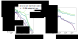
\includegraphics[width=\textwidth]{figures/5_downstream}
		\phantomsubcaption
		\label{fig:downstream_a}	
	\end{subfigure}
	\begin{subfigure}[t]{0\linewidth}
		\phantomsubcaption
		\label{fig:downstream_b}
	\end{subfigure}
	\caption{\footnotesize{\textbf{Front-end adaptation enhances odor recognition by the \textit{Drosophila} olfactory circuit.} 
	\textbf{A} Accuracy of binary classification by odor valence, as a function of the number of distinct odor identities classified by the trained network (concentrations span 4 orders of magnitude), in systems with only ORN adaptation, only divisive normalization, both or neither. \textbf{B} Same as (A) but now classifying odors  by identity.
	}}
	\label{fig:downstream}
\end{figure}


Previous studies have characterized various neural mechanisms that help preserve combinatorial codes. 
Lateral inhibition between glomeruli helps tame saturation and boost weak signals~\cite{divisive_normalization}. %ORNs exhibiting both excitatory and inhibitory responses to odorants can increase coding capacity by exploiting response bidirectionality~\cite{Cao_Tu_WL}. In vertebrates, G-protein-coupled chemoreceptors rather than Orco-coupled cation channels, antagonism among odorants may help maintain response sparsity~\cite{reddy2017antagonism}. 
The sparse degree of connectivity to either the olfactory bulb (vertebrates) or mushroom body (insects) %(in the fly each KC receives connections from only $\sim$7 AL glomeruli) 
may also be precisely tuned to optimize the capacity to learn associations~\cite{litwinkumar}. In this work, we find that some of these downstream features act in concert with front-end dynamic adaptation in maintaining representations of odor identity.

Other studies have implicated the unique temporal patterns of neural response as signatures of odor identity~\cite{stopfer_temporal_model, multiple_timescales_stopfer, stopfer_nat_neuro, stopfer_temporal_channel}. ORN and projection neuron time traces form distinct trajectories in low-dimensional projections, and cluster by odor identity, {\color {blue} 
much as we have found here for static responses at different concentrations
}
(Fig.~\ref{fig:coding}). In locusts PNs, the trajectories elicited by foreground odors when presented in distinct backgrounds exhibit some degree of overlap; though partial, these overlaps were nonetheless sufficient to maintain background-invariant decoding from Kenyon cell responses~\cite{coding_background}. It was therefore suggested that background filtering likely occurs at the level of ORNs themselves~\cite{coding_background}. Likewise, in our framework, temporal coding is implicit: because the input nonlinearity depends on the diversity of binding affinities, %strength of feedback onto Or-Orco activation depends on an ORN's unique response characteristics, 
odor signals are naturally formatted into temporal patterns that are both odor- and ORN-specific  (Figs.~\ref{fig:tuning_curves_d}-\ref{fig:tuning_curves_e}). Further, the short required memory timescales  ($\tau_{\textup M} \sim \tau \sim 250$ ms) suggest that only brief time windows are needed for accurate odor identification, consistent with previous findings~\cite{stopfer_nat_neuro, coding_background}. Moreover, we find that front-end adaptation enhances the robustness of other combinatorial coding schemes, such as primacy coding~\cite{primacy_coding}, which relies on the temporal order of ORN activation but not absolute firing rate (Fig.~\ref{fig:primacy_coding}).

In the well-characterized chemosensory system of bacterial chemotaxis, Weber Law adaptation is enacted through a feedback loop from the output activity of the receptor-kinase complexes onto the enzymes modifying receptor sensitivity~\cite{EmonetReview}. It is interesting that some aspects of this logic are also present in ORNs: although the molecular players are different 
{\color {blue} 
(and still largely unknown, though likely involving calcium channel signaling~\cite{cao_WL}), 
}
it has been shown that transduction activity feeds back onto the sensitivity of Or-Orco ligand-gated cation channels, enabling the Weber-Fechner relation~\cite{nagel_wilson_biophysical,srinivas_elife,cao_WL}. 
That this adaptation mechanism appears to act similarly across ORNs~\cite{srinivas_elife,martelli,cao_WL} suggests the possible involvement of the universal co-receptor Orco, whose role in long-term adaptation has recently been reported~\cite{getahun2013insect,getahun2016intracellular,Guo_Smith}. Further, the identification of 4 subunits comprising the Orco-Or ion channel suggest that generic Or/Orco complexes may contain multiple odorant binding sites, which when included in our model supports our general findings (Fig~\ref{fig:SI_mult_binding}).

Weber Law ensures that sensory systems remain in the regime of maximum sensitivity, broadening dynamic range and maintaining information capacity~\cite{adaptation_fairhall}.
%, laughlin, deweese_adaptation}. 
%Doing so requires matching sensory response to attributes of the environment, either by adapting to specific stimuli or to stimuli statistics~\cite{adaptation_fairhall}. 
For a single-channel system, this requires matching the midpoint of the dose-response curve to the mean ligand concentration~\cite{information_theory_adaptation}, a strategy which may fail in multi-channel systems with overlapping tuning curves: adaptation to one signal could inhibit identification of others, if the signals excite some but not all of the same sensors, as in Fig.~\ref{fig:tuning_curves_g}. 
Our results show that this strategy is still largely functional. In CS decoding, this can be traced to the observation that accuracy is guaranteed when sufficiently distinct odor identities produce sufficiently distinct ORN responses, a condition known as the restricted isometry property~\cite{CS_tao}. Indeed, the Weber-Fechner scaling increases the likelihood that this property  is satisfied, beyond that in the non-adaptive system (SI text and Fig.~\ref{fig:SI_HIT_eigs}-Fig.~\ref{fig:SI_IHT_est}). Still, restricted isometry does not require that response repertoires are \textit{invariant} to environmental changes. That is, even if the subset of active ORNs were concentration-dependent, odors could still in principle be fully reconstructible by CS.
Nonetheless, our results in t-SNE clustering (Fig.~\ref{fig:coding}), primacy coding  (Fig.~\ref{fig:primacy_coding_b}-\ref{fig:primacy_coding_c}), and odor classification (Fig.~\ref{fig:downstream}) suggest that some signature of response invariance emerges as a natural byproduct of front-end adaptation. Together, this implies that Weber Law adaptation, whether required by the olfactory circuit for precise signal reconstruction (as in CS) or for developing odor associations (as in classification), can play an integral part in maintaining combinatorial codes amid changing environmental conditions.

%Viewing sensory systems as input/output machines, the role of adaptation is therefore to maintain information capacity in dynamic environments~\cite{information_theory_adaptation}. 
%For a single-channel, information capacity is increased by matching the midpoint of the nonlinear dose-response curve, where sensitivity is highest, to mean ligand concentration according to Weber-Fechner law~\cite{information_theory_adaptation}. 

%universal adaption: adaptation to one odor could adversely affect identification of a new odor, if the latter excites some but not all of the same ORNs. In compressed sensing, signal reconstruction requires that odor signals produce sufficiently distinct responses, a mathematical condition known as the restricted isometry property. Our results show that front-end adaptation  preserves this property, helping maintain combinatorial representations of odor identity despite the broad overlaps in the tuning curves of the receptors.



\section*{Acknowledgements}

NK was supported by a postdoctoral fellowship through the Swartz Foundation and through an NRSA postdoctoral fellowship through the NIH BRAIN Initiative under award number 1F32MH118700. TE was supported by NIH R01 GM106189. We thank Damon  Clark, John Carlson, Mahmut Demir, Srinivas Gorur-Shandilya, Henry Mattingly, and Ann Hermunstad for comments on the manuscript. 

\section*{Author Contributions}
N.K. and T.E. conceived the project, analyzed the results, and wrote the manuscript. N.K. performed all calculations. T.E. supervised the project.

\section*{Declaration of Interests}
The authors declare no competing interests.




%%%%%%%%%%%%%%%%%%%%%%%%%%%%%%%%%%%%%%%%%%%%%%%%%%%%%%%%%%%%%%%%%
%%%%%%%%%%%%	   	           METHODS                %%%%%%%%%%%
%%%%%%%%%%%%%%%%%%%%%%%%%%%%%%%%%%%%%%%%%%%%%%%%%%%%%%%%%%%%%%%%%




\section*{Methods}



\textit{Adaptive ORN model} \\


We model an odor as an $N$-dimensional vector ${\mathbf s=[ s_1,...,s_N]}$, where $s_i > 0$ are the concentrations of individual volatile molecules (odorants) comprising the odor. 
The olfactory sensory system is modeled as a collection of $M$ distinct Or/Orco complexes indexed by the sub index $a=1,...,M$, each of which can be bound with any one of the odorant molecules, and can be either active (firing) or inactive (quiescent). At first we assume there is one binding site per complex; this will be generalized to many sites. We consider the binding and activation processes to be in equilibrium, assigning each state a corresponding Boltzmann weight, where the zero of energy is set by the unbound, inactive state $\textup{C}_a$. These weights are:

\begin{align}
    &\textup{C}_a        &&      1 \nonumber \\
    &\textup{C}^*_a      &&      \exp({-\beta \epsilon_a}) \nonumber \\
    &\textup{C}_a\textup{:}s_i     &&      \exp({-\beta(-E_{ai}  - \mu_{i})}) \nonumber \\
    &\textup{C}^*_a\textup{:}s_i   &&      \exp({-\beta(-(E_{ai}^* - \epsilon_a) - \mu_{i}}),
\end{align}
where $\epsilon_a$ (assumed positive) is the free energy difference between the active and inactive conformation of the unbound receptor, and $E_{ai}$ and $E_{ai}^*$ are the free energy differences (assumed positive) between the unbound and bound state for the inactive and active receptor, respectively. $\mu_{i}=\mu_0+\beta^{-1}\log(s_i/s_0)$ is the chemical potential for odorant species $i$ in terms of a reference chemical potential $\mu_0$ at concentration $s_0$, $s_0\exp(-\beta \mu_0) = s_i\exp(-\beta \mu_{i})$, which can be traded for the thermodynamic-relevant disassociation constants $K_{ai}^{-1} = K_{\textup{D}, ai} = s_0 e^{\beta (-E_{ai} - \mu_0)}$. 

Adding up contributions from all $i$ odorants, the active fraction is:
\begin{align}
A_a &= \frac{
    \textup{C}^*_a + \sum_i \textup{C}^*_a\textup{:}s_i}{\textup{C}^*_a + \sum_i \textup{C}^*_a\textup{:}s_i + \textup{C}_a + \sum_i \textup{C}_a\textup{:}s_i} \nonumber \\
	&= \left(1 + \frac{\textup{C}_a + \sum_i \textup{C}_a\textup{:}s_i}
	{\textup{C}^*_a + \sum_i \textup{C}^*_a\textup{:}s_i} \right)^{-1} 
	\nonumber \\
    &= \left(1 + e^{\epsilon_a}\frac{1 + \mathbf{K}_a\cdot\mathbf{s}(t)}{1 + \mathbf{K}^*_a\cdot\mathbf{s}(t)}
    \right)^{-1}, 
    \tag{\ref{eq:steady_state_act_OR}}
\end{align} 
where we have expressed free energies in units of $k_B T=\beta^{-1}$ for notational convenience.

This expression can be generalized for the case of multiple, independent binding sites through some simple combinatorial factors. Consider first an odorant $i$ which can bind one of two locations on receptor $a$. There are then 4 possible inactive states: both sites unbound, site 1 bound, site 2 bound, both sites bound. Combined with the active states, there are therefore 8 states for odorant $i$ and receptor $a$, with energies: 

\begin{align}
& \textup{active}  
&& \{1, \quad -E_{ai} - \mu_i, \nonumber \\
    &&&\quad -E_{ai} - \mu_i, 
    \quad -2E_{ai} - 2\mu_i\} \nonumber \\
& \textup{inactive}  
&& \{\epsilon_a, 
    \quad -(E^*_{ai}  - \epsilon_a) - \mu_i, 
    \nonumber \\
    &&&\quad -(E^*_{ai}  - \epsilon_a) - \mu_i,
    \nonumber \\ 
    &&&\quad -(2E^*_{ai}  - \epsilon_a) - 2\mu_i\} 
\end{align}

In the active fraction, Eq.~\ref{eq:steady_state_act_OR}, the Boltzmann factors combine through the binomial theorem, giving (for a single odorant environment $i$):

\begin{align}
&A_a(\textup {odorant }i \textup{, 2 binding sites})  \nonumber \\
    &\qquad =\left[1 + e^{\epsilon_a}\left(\frac{1 + \mathbf{K}_a\cdot\mathbf{s}(t)}{1 + \mathbf{K}^*_a\cdot\mathbf{s}(t)}\right)^2\right]^{-1}.
\end{align} 

This expression generalizes for an arbitrary number of odorants and independent binding sites through the appropriate combinatorial factors, giving an active fraction of
\begin{align}
&A_a(N \textup { odorants}, R \textup { binding sites}) \nonumber \\
    &\qquad = \left[1 + e^{\epsilon_a}\left(\frac{1 + \mathbf{K}_a\cdot\mathbf{s}(t)}{1 + \mathbf{K}^*_a\cdot\mathbf{s}(t)}\right)^R\right]^{-1}. 
\end{align} 




To generate ORN time traces, equations~\ref{eq:steady_state_act_OR}-\ref{eq:adaptation_dynamics} are integrated numerically using the Euler method with a 2 ms time step. For ORN firing (Eq.~\ref{eq:firing_machinery}), $h(t)$ is bi-lobed~\cite{martelli}: $h(t) = Ap_{\textup{Gam}}(t; \alpha_1, \tau_1) - Bp_{\textup{Gam}}(t; \alpha_2, \tau_2)$, $A = 190$, $B = 1.33$,  $\alpha_1=2$, $\alpha_2=3$, $\tau_1 = 0.012$, and $\tau_2 = 0.016$, where $p_{\textup{Gam}}$ is the pdf of Gamma($\alpha$, $1/\tau$). Nonlinearity $f$ is modeled as a linear rectifier with 5 Hz threshold. \\




\textit{Derivation of ORN gain} \\


{\color {blue} 

Weber's Law states that the gain, or differential response, of the receptor activity $A_a$ scales with the mean odor concentration $\bar s_i$. To show how this is satisfied in our model, we consider the response, Eq.~\ref{eq:steady_state_act_OR}, to a signal $\mathbf{s} = \bar {\mathbf{s}} + \Delta \mathbf{s}$, where $\Delta \mathbf s$ consists of only a small fluctuation in the $i$th component $\Delta s_i < |\bar s_i|$ about the mean. We derive the change in response to fluctuation $\Delta s_i$ for general $\beta$ from 0 (Weber's law) to 1 (no adaptation).

First we write the activity in the form:

\begin{align}
A_a &= (1 + e^{F_a})^{-1},
\end{align}

where

\begin{align}
F_a = \epsilon_a(\bar {\mathbf s}) + 
    \ln\left(\frac
    {1 + \mathbf{K}_a\cdot {\mathbf{s}}} 
    {1 + \mathbf{K}^*_a\cdot {\mathbf{s}}} 
    \right).
\end{align}

where $\epsilon_a(\bar {\mathbf s})$ is given by Eq.~\ref{eq:beta}.
Then, assuming $1/\mathbf{K}^*_a \ll s_i \ll 1/\mathbf{K}_a$, the change in response from the adapted level $A_a(\bar {\mathbf s})$ is

\begin{align}
    A_a(\mathbf s) - A_a(\bar {\mathbf s}) = {\Delta A_a}%\big|_{\bar {\mathbf s}} 
    &= \frac{dA_a}{dF_a}\frac{dF_a}{ds}\bigg|_{\bar {\mathbf s}}\Delta s_i \nonumber \\
    &= -\frac{e^{F_a}}{(1 + e^{F_a})^2}\bigg|_{\bar {\mathbf s}}
    \left(\frac{-K^*_{ai}}{\mathbf{K}^*_a\cdot \bar {\mathbf{s}}}\right) \Delta s_i.
\end{align}

We use Eq.~\ref{eq:beta} to evaluate $e^{F_a}$ at $\bar {\mathbf s}$, obtaining:

\begin{align}
    e^{F_a} &\approx \frac{1 - A_{0a}}{A_{0a}}
    (\mathbf{K}^*_a\cdot \bar {\mathbf{s}})^{-\beta},
\end{align}

whereby

\begin{align}
    \frac{\Delta A_a}
    {\Delta s_i}%\bigg|_{\bar {\mathbf s}}
    &= 
    \frac{
    \frac{1 - A_{0a}}{A_{0a}}
    (\mathbf{K}^*_a\cdot \bar {\mathbf{s}})^{-\beta}
    }
    {(1 + \frac{1 - A_{0a}}{A_{0a}}
    (\mathbf{K}^*_a\cdot \bar {\mathbf{s}})^{-\beta})^2
    }
    \left(\frac{K^*_{ai}}{\mathbf{K}^*_a\cdot \bar {\mathbf{s}}}\right)\nonumber \\
    &=\frac{(1 - A_{0a})A_{0a}K^*_{ai}}
    {
    [
    A_{0a}(\mathbf{K}^*_a\cdot 
    \bar {\mathbf{s}})^{\frac{1+\beta}{2}}
    +
    (1 - A_{0a})(\mathbf{K}^*_a\cdot 
    \bar {\mathbf{s}})^{\frac{1-\beta}{2}}
    ]^2
    }.
    \label{eq:full_gain_eq}
\end{align}


For $\beta = 0$ (the fully adaptive case) and a single odorant, this expression for the gain reduces to $(1 - A_{0a})A_{0a}/s_i$. For small $\beta$, and given $A_{0a} \simeq 0.1$ (corresponding to 30 Hz on a 300 Hz firing rate scale), the denominator is dominated by the $1 - A_{0a}$ term, giving:

\begin{align}
    \frac{\Delta A_a}
    {\Delta s_i}\bigg|_{(\beta \ll 1)}
    &=\frac{A_{0a}K^*_{ai}}
    {(1 - A_{0a})
    (\mathbf{K}^*_a\cdot 
    \bar {\mathbf{s}})^{1 - \beta}
    }.
\end{align}

The implication of this is that the gain scaling of the inverse mean intensity, which is $1$ for perfect adaptation (gain $\sim (1/s_i)^1$), is now sublinear. Thus, when Weber's Law is weakly broken, the gain still reduces with mean odor intensity, but not as quickly. \\

}

\textit{t-SNE dimensionality reduction} \\



For t-SNE dimensionality reduction~\cite{tsne}, ORN responses were generated for odor signal combinations consisting of 1 (among 10) distinct sparse foreground odors A atop 1 (among 50) distinct sparse background odors B, for Fig.~\ref{fig:coding_b}.  Fig.~\ref{fig:coding_c} plots responses for 10 odors at 40 concentrations spanning 4 decades, atop a random sparse background odor of similar magnitude. For adaptive systems, $\epsilon_a$ were set to their fully adapted values to the background odor, given by Eq.~\ref{eq:beta}, with $\beta = 0$. For Figs.~\ref{fig:coding_d}, for each $\beta$, we averaged the silhouette score $H$ (defined precisely below) over 5 different trials, each trial with a different seed for randomly choosing the odor identities. 

{\color {blue} 

To calculate performance of clustering in the t-SNE plots, we use the silhouette score $H$~\cite{silhouette_score}, which is a function of the 2D Euclidean distance $d(i, j| m, n)$ between the point $p_{ij}$ representing odor $s_i$ on background $b_j$ and the point $p_{mn}$ representing odor $s_m$ on background $b_n$. For each $p_{ij}$, we define $a(ij)$ as:

\begin{align}
    a(ij) = \frac{1}{1-N_i}\sum_{n \in C_i} d(i, j| i, n)
\end{align}

where $C_i$ is the set of all points in cluster $i$, i.e. with foreground $i$. This quantifies the average distance of $p_{ij}$ to other points in the same cluster, i.e. with the same foreground but different backgrounds. We next define $b(ij)$ as:

\begin{align}
    b(ij) = \min_{m \ne i}
    \frac{1}{N_m}\sum_{n \in C_m} d(i, j| m, n),
\end{align}

where the sum is taken over all points $p_{mn}$ in cluster $m$ -- i.e. with foreground $m$ not equal to $i$ -- and the minimum is taken over all clusters $m$. This quantifies the average distance from $p_{ij}$ to the points in its "nearest neighbor" cluster.
Then, $H$ is defined as:

\begin{align}
    H = \langle \frac{a(ij) - b(ij)}{\max\{a(ij), b(ij)\}}
    \rangle_{ij},
\end{align}

where the average is taken over all points $ij$ in the t-SNE plot. $H$ is nearer to 1 when points cluster by foreground, and is near zero or slightly negative when the clusters cannot be disambiguated. \\
}


\textit{Compressed sensing decoding of ORN responses} \\


%Mutual information was calculated from 1000 randomly chosen sparse odor identities ($K = 4$ for both odor A and odor B), with noise $\sigma \sim \mathcal{N}(0, \textup{1e-3})$ added to $A_a$. 


Compressed sensing (CS) addresses the problem of determining a sparse signal from a set of linear measurements, when the number of measurements is less than the signal dimension. Specifically, it is a solution to 

\begin{align}
\mathbf y = \mathbf D\mathbf x,
\label{eq:CS_constraints}
\end{align} 

where $\mathbf x \in \mathbb{R}^N$ and $\mathbf y\in \mathbb{R}^M$ are vectors of signals and responses, respectively, and $\mathbf D$ is the measurement matrix. Since measurements are fewer than signal components, then $M < N$, whereby $\mathbf D$ is wide rectangular and so Eq.~\ref{eq:CS_constraints} cannot be simply inverted to produce $\mathbf x$. The idea of CS is to utilize the knowledge that $\mathbf x$ is sparse, i.e. only $K$ of its components, $K \ll N$ are nonzero. Both the measurements and sparsity are thus combined into a single constrained optimization routine:

\begin{align}
\hat x_i = \textup{argmin} \sum_i^N |x_i| \quad \textup{such that } \mathbf y = \mathbf D\mathbf s
\label{eq:CS}
\end{align}

where $\hat x_i$ are the optimal estimates of the signal components and the sum, which is known as the $L_1$ norm of $\mathbf x$, is a natural metric of sparsity~\cite{CS_donoho}. 

The $L_1$ norm is a convex operation and the constraints are linear, so the optimization has a unique global minimum. To incorporate the nonlinear response of our encoding model into this linear framework, we assume that the responses are generated through the full nonlinear steady state response, Eq.~\ref{eq:steady_state_act_OR}-~\ref{eq:firing_machinery}, but that the measurement matrix $\mathbf D$ needed for decoding uses a linear approximation of this transformation.  Expanding Eq.~\ref{eq:firing_machinery} around $\bar{\mathbf s} = \mathbf s - \Delta \mathbf s$ gives

\begin{align}
\Delta r_a(t) &= r_a(\mathbf s(t)) - r_a(\bar{\mathbf s}(t)) \nonumber \\
\Delta r_a(t) &= \int^t d\tau h(t- \tau)\sum_i^N\frac{dA_{ai}}{ds_i}\bigg|_{\bar{\mathbf s}}\Delta s_i \label{eq:CS_dAct_approx}
\end{align}

where 

\begin{align}
r_a(\mathbf s_0) &= \int^t d\tau h(t- \tau)\sum_i^NA_{0a} 
\label{eq:CS_r_approx} 
\end{align}

and where $\frac{dA_{ai}}{ds_i}\big|_{\bar{\mathbf s}}$ is given by the right-hand side of Eq.~\ref{eq:full_gain_eq} with $\beta = 0$. Eqs.~\ref{eq:CS_dAct_approx} and~\ref{eq:CS_r_approx} hold only for integrands above 5 Hz (and are zero below), as per the linear rectifier $f$. We assume that the neural decoder has access to background $\bar{\mathbf s}$, presumed learned (this assumption can be relaxed; see below), and to  the linearized response matrix, Eq.~\ref{eq:full_gain_eq}, but must infer the excess signals $\Delta s_i$ from excess ORN firing rates $\Delta r_a(t)$. Thus, this corresponds to the CS framework (Eq.~\ref{eq:CS})  via $\Delta \mathbf {r} \rightarrow \mathbf y$, $\Delta \mathbf s \rightarrow \mathbf x$, and $dA_{ai}/{ds_i}\big|_{\bar {\mathbf s}} \rightarrow \mathbf D$. We optimize the cost function in Eq.~\ref{eq:CS} using sequential least squares programming, implemented in Python through using the scientific package SciPy. 



For our simulations, we let sparse components $s_i$ be chosen as $s_i = \bar s_i + \Delta s_i$, where $\bar s_i= s_0$ and $\Delta s_i \sim \mathcal {N} (s_0/3, s_0/9)$. The measurement matrix $\mathbf D$ depends on the free energy differences $\epsilon_a$. For static stimuli, $\epsilon_a$ equals the fixed point of Eq.~\ref{eq:adaptation_dynamics} in response to the background stimulus with $\beta = 0$. For fluctuating stimuli, $\epsilon_a$ is updated in time by continuously integrating  $r_a(t)$, via Eqs.~\ref{eq:adaptation_dynamics} and~\ref{eq:firing_machinery}; thus, only knowledge of the response $r_a(t)$ are needed by the decoder. 
{\color {blue} 
To quantify decoding accuracy, we treat the zero and nonzero components of the sparse odor vector separately. We demand that the $K$ nonzero components $\hat s_i$ of the estimated sparse vector are within 25\% of their true values $s_i$, and that the $N - K$ zero components are estimated less than $10\%$ of $s_0$. Together, this ensures that the odorants comprising the odor mixture are estimated sufficiently close to their concentrations, and that the remaining components are sufficiently small. Odor signals $\mathbf s$ are considered correctly decoded if both of these conditions are satisfied for all components $s_i$. The relatively lax accuracy demanded on the nonzero components is to prevent oversensitivity on the unavoidable errors introduced by linearization. Qualitatively, our findings are robust to these choices. 
}
The naturalistic odor signal (Fig.~\ref{fig:decoding_d}) was generated by randomly varying flow rates of ethyl acetate and measuring the concentration with a photo-ionization detector~\cite{srinivas_elife}. Statistics mirroring a turbulent flow~\cite{celani} were verified (Fig.~\ref{fig:SI_odor_stats}). \\


\textit{Iterative hard thresholding (IHT) and the restricted isometry property in compressed sensing} \\


The purpose of response linearization (Eq.~\ref{eq:CS_dAct_approx}) is simply to apply compressed sensing reconstruction directly using linear programming, without worrying about issues of local minima in Eq.~\ref{eq:CS}. This allows us to isolate the impact  of Weber Law adaptation from the particularities of the numerics. An alternate technique for compressed signal reconstruction, \textit{iterative hard thresholding} (IHT), does not minimize the constrained $L_1$ norm directly, rather applying a hard threshold to an iteratively updated signal estimate~\cite{IHT}. IHT can be generalized straightforwardly to nonlinear constraints, and would actually dispense with the need for a learned background $\bar{\mathbf s}$, simply initializing the iterations from $\bar{\mathbf s} = \mathbf 0$. Remarkably, this technique works quite well even for non-linear measurements~\cite{nonlin_CS}. We demonstrate the applicability of the IHT algorithm to our odor decoding system in Fig.~\ref{fig:SI_IHT_est}, which reproduces qualitatively the findings in the main text. For these calculations, no background odor was assumed, each iterative decoding being initialized $\bar {\mathbf s} = \mathbf {0}$.

IHT provides an alternate computational technique of nonlinear CS, which could be used to both extend and verify our results. Further, it allows us to illustrate why Weber Law adaptation maintains signal reconstruction fidelity in our olfactory sensing model. Like CS using $L_1$-norm minimization, IHT exhibits amenable reconstruction and convergence properties under the guarantee of the so-called restricted isometry property (RIP)~\cite{CS_tao_2}. Loosely, RIP measures how closely a matrix operator resembles an orthogonal transformation when acting on sparse vectors. The degree to which RIP is satisfied can be understood in terms of the spectrum of a measurement matrix $\mathbf D$. In particular, if $\lambda_i$ are the eigenvalues of $\mathbf {D}_k^T\mathbf {D}_k$, where $\mathbf D_k$ is any $k \times m$ submatrix of $\mathbf D$, and 

\begin{align}
    1 - \delta_k \leq \lambda_{min} \leq \lambda_{max} \leq 1 + \delta_k
\end{align}

is satisfied for some $\delta_k$, then $\mathbf D$ satisfies the RIP with constant $\delta_k$. Plainly, the RIP states that the eigenvalues of $\mathbf {D}_k^T\mathbf {D}_k$, when acting on $k$-sparse vectors, are centered around 1. Thus, to intuit why signal reconstruction breaks down in the non-adaptive sensing system, we can investigate the eigendecomposition of various linearizations of the measurement matrix. We do this now, starting with a brief description of the IHT.

In the linear setting, IHT seeks sparse signals via the following iterative procedure~\cite{IHT}:
\begin{align}
    \mathbf{x}_{k + 1} = H_K(\mathbf{x}_k + \mu\mathbf{D}^T(\mathbf {x}_k + (\mathbf y - \mathbf D\mathbf {x}_k)))
    \label{eq:IHT}
\end{align}
where $\mathbf{x}_k$ is the $k$th estimate of the sparse signal $\mathbf{x}$, $\mu$ is a step size for the iterations, and $\mathbf y$, $\mathbf D$ are as defined above. $H_k(\cdot)$ is a thresholding function which sets all but the largest $K$ values of its argument to zero. The nonlinear extension to IHT is~\cite{nonlin_CS}:

\begin{align}
    \mathbf{x}_{k + 1} = H_K(\mathbf{x}_k + \mu\mathbf{D}_{\mathbf x_n}^T(\mathbf {x}_k + (\mathbf y - D(\mathbf {x}_k)))),
    \label{eq:IHT_NL}
\end{align}

where $D$ is a nonlinear sensing function and $\mathbf{D}_{\mathbf x_n}$ is a linearization of $D$ about the point $\mathbf x_n$. Reconstructibility for $k$-sparse signals is guaranteed if $\mathbf{D}_{\mathbf x_n}$ satisfies RIP for all $\mathbf x_n$ and all $k$-sparse vectors~\cite{IHT}. To get a sense of how this is preserved in the adaptive system, we calculate the eigenvalues for 1000 choices of $\mathbf x_n$, acting on random signals of given sparsity $K$ (Fig.~\ref{fig:SI_HIT_eigs}). Since the RIP is sensitive to constant scalings of the measurement matrix (while the actual estimation problem is not), we scaled all columns of $\mathbf{D}_{\mathbf x_n}$ to norm unity~\cite{using_IHT}. This normalizes the eigenvalues of $\mathbf{D}^T_{\mathbf x_n}\mathbf{D}_{\mathbf x_n}$ to center near unity before calculating the eigendecomposition, allowing us to assess the degree to which the RIP is satisfied. This scaled matrix can be used directly in Eq.~\ref{eq:IHT_NL}~\cite{nonlin_CS,using_IHT}. The spectra of these matrices indicates that the RIP becomes far more weakly satisifed in the non-adaptive system than in the adaptive one, for sufficient odor complexity and intensity. \\

\textit{Network model and classification} \\


For the network model, the AL-to-MB connectivity matrix $\mathbf {J}_1$, is chosen such that  each KC connects pre-synaptically to 7 randomly chosen AL glomeruli~\cite{litwinkumar,abbott_axel}. The results shown in Fig.~\ref{fig:downstream} are an average of 10 distinct instantiations of this random topology. The $Z=2500$ KCs are then connected by a matrix $\mathbf J_2$ to a readout layer of dimension $Q$, where $Q=2$ for binary and $Q=N_{\text{ID}}$ for multi-class classification. Both AL-to-MB and MB-to-readout connections are perceptron-type with rectified-linear thresholds. The weights of $\mathbf J_1$ and $\mathbf J_2$ are chosen randomly from $\sim \mathcal{N}(0, 1/\sqrt{7})$ and $\sim \mathcal{N}(0, 1/\sqrt{Z})$, respectively. Only the $\mathbf J_2$ and the MB-to-output thresholds are updated during supervised network training, via logistic regression (for binary classification) or its higher-dimensional generalization, the softmax cross entropy (for multi-class classification).
\bibliography{bibliography}






%% SI






\onecolumngrid

\pagebreak


\renewcommand\thefigure{\ref{fig:coding}--figure supplement 1}  



\begin{figure}
\centering
\includegraphics[width=\linewidth]{figures/2_coding_representation_SI}
\caption{
{\color{blue}
t-SNE projections for non-adaptive ($\beta = 1$) and adaptive ($\beta = 0$) systems, when background firing rates depend on ORN identity. Background active fractions $A_{0a}$ are chosen normally with mean 0.1 and deviation 0.03, corresponding to background firing rates around of $\simeq$ 20-40 Hz. 
}
}
\label{fig:SI_coding}
\end{figure}



\renewcommand\thefigure{\ref{fig:coding}--figure supplement 2}  




\begin{figure}
\centering
\includegraphics[width=0.8\linewidth]{figures/2_coding_representation_SI_2}
\caption{
Front-end adaptive feedback preserves information capacity of the ORN sensing repertoire. 
\textbf{A} 
Mutual information between signal $\mathbf s(t)=\mathbf s_A(t)+\mathbf s_B(t)$ and response $\mathbf r(t)$ is calculated at various points in time $t$ for an odor environment consisting of two step odors, A and B. Odor A, with concentration $\mathbf s_A(t)$, turns on at time $t_A$ and a odor B, with concentration $\mathbf s_B(t)$, turns on at some later time $t_B$. Both odors have similar intensities $\sim s_0$ and similar molecular complexity ($k = 4$). 
\textbf{B} Mutual information as a function of $s_0$ for the non-adaptive system, respectively, at different time points after $t_A$, corresponding to the dots in A. The mutual information carried by distinct ORNs is represented by the shaded region; their average is plotted by the heavy line. In the non-adaptive system, the mutual information peaks in the regime of high sensitivity after the arrival of odor A (purple, blue), and shifts leftward with the onset of odor B (teal, green). The leftward shifts occurs since stronger signals are more prone to response saturation (compromising information transfer) as odor B arrives. 
\textbf{C} Same as \textbf{B}, now for the adaptive system. The MI mimics the non-adaptive case at the onset of odor A, before adaptation has kicked in (purple). As the system adapts and responses decrease toward baseline, previously saturating signal intensities now cross the regime of maximal sensitivity, which therefore shifts rightward to higher $s_0$ (dark blue). Much later, but before the arrival of odor B, the ORNs that responded now fire at a similar  adapted firing rate $\sim 30$ Hz, irrespective of odor identity, so the mutual information drops to zero. However, having now adjusted its sensitivity to the presence of odor A, the system can respond appropriately to odor B: the MI at $t_B$ is nearly 6 bits across decades of concentration immediately following $t_B$ (green). 
}
\label{fig:SI_MI}
\end{figure}



\renewcommand\thefigure{\ref{fig:decoding}--figure supplement 1}  


\begin{figure}
\centering
\includegraphics[width=0.6\textwidth]{figures/temporal_broad_tA.pdf}
\caption{Decoding accuracy for system with broader distribution of adaptive timescales $\tau$.
\textbf{A} Distribution of timescales for all ORNs $a$ (purple dots). Here, $\tau_a \sim = 10^X$ where $\tau = 250$ ms as in the main text and $X \sim \mathcal N(0, 0.2)$. 
\textbf{B}  Individual plots show the percent of accurately decoded odor whiffs (same fluctuating odor signal used in the main text) as a function of background odor intensity, for the non-adaptive (blue) and adaptive (red) systems, for different $\tau_M$ (line shades). Plots are arrayed by the complexity of the naturalistic signal (column-wise) and the complexity of the background odor (row-wise).
}
\label{fig:SI_broad_tA}
\end{figure}



\renewcommand\thefigure{\ref{fig:decoding}--figure supplement 2}  


\begin{figure}
\centering
\includegraphics[width=0.8\textwidth]{figures/broad_A0}
\caption{Benefits conferred by Weber-Fechner adaptation remain for a broader distribution of baseline firing rates $A_{0a}$, now assumed to be ORN-dependent and chosen from a normal distribution.
\textbf{A} Distribution of $A_{0a}$.
\textbf{B} Decoding accuracy of foreground odors in the presence of background odors.}
\label{fig:SI_broad_A0}
\end{figure}


\renewcommand\thefigure{\ref{fig:decoding}--figure supplement 3}  


\begin{figure}
\centering
\includegraphics[width=0.8\textwidth]{figures/2_binding_sites}
\caption{Benefits conferred by Weber-Fechner adaptation remain for 2 binding sites per receptor. This might conceivably occur in insect olfactory receptors, heterotetramers consisting of 4 Orco/Or subunits that gate a central ion channel pathway~\cite{orco_structure}. Plotted is the decoding accuracy of foreground odors in the presence of background odors.
}
\label{fig:SI_mult_binding}
\end{figure}


\renewcommand\thefigure{\ref{fig:decoding}--figure supplement 4}  


\begin{figure}
\centering
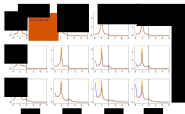
\includegraphics[width=0.95\textwidth]{figures/HIT_eigs}
\caption{Eigenvalue distribution of $\mathbf{A}_{\mathbf x_n}^T\mathbf{A}_{\mathbf x_n}$, where $\mathbf{A}_{\mathbf x_n}$ is a $m \times k$ submatrix of the  column-normalized linearized ORN response matrix $\mathbf{A}$, evaluated at the linearization point $\mathbf x_n$. Note that $\mathbf x_n$ is $k$-sparse, but its components do not necessarily align with the $k$ columns chosen for the sub-matrix. Eigenvalues are calculated for the adaptive (orange) and non-adaptive (blue) systems, for 1000 randomly chosen linearization points $\mathbf x_n$ and submatrices. Plots are arranged for various odor sparsities (by row) and odor intensities (by column). The restricted isometry property is satisfied when the eigenvalues lie between 0 and 2 (black vertical line), and is more strongly satisfied the more centered the distribution is around unity. The increase in near-zero eigenvalues for the non-adaptive system at higher odor complexities and intensities (lower right plots) indicates the weaker fulfillment of the restricted isometry property for thhse signals, and leads to higher probability of failure in compressed sensing signal reconstruction.
}
\label{fig:SI_HIT_eigs}
\end{figure}


\renewcommand\thefigure{\ref{fig:decoding}--figure supplement 5}  


\begin{figure}
\centering
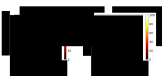
\includegraphics[width=0.8\textwidth]{figures/HIT_est}
\caption{Decoding of odor signals (no background odors) using the IHT algorithm~\cite{IHT, nonlin_CS} qualitatively reproduces the results from the main text, which used traditional CS with background linearization. In the adaptive case, IHT actually exhibits superior accuracy to traditional CS, though IHT demands more compute time. The results here show odor decoding accuracy for sparse odor signals of given complexity and intensity, averaged over 10 distinct identities. Odors are considered accurately decoded if the $K$ sparse components are estimated within 25\% and the components not in the mixture are estimated below 10\% of $s_0$. The iterative algorithm was initialized at $ \hat{ \mathbf x} = \mathbf 0$ and run forward until $ \hat{ \mathbf x}$ was stationary, or 10000 iterations were reached. Step size $\mu$ in Eq.~\ref{eq:IHT_NL} was set to $s_0/20$. At each step, the linearized response ($\mathbf{A}_{\mathbf x_n}$ in Eq.~\ref{eq:IHT_NL}) was evaluated at the result of the previous iteration. IHT also requires an assumption on the number of components in the mixture (which defines  $H_K(\cdot )$ in Eq.~\ref{eq:IHT_NL}); here, that was set to twice the actual sparsity of true signal. 
}
\label{fig:SI_IHT_est}
\end{figure}


\renewcommand\thefigure{\ref{fig:decoding}--figure supplement 6}  



\begin{figure}
\centering
\includegraphics[width=0.6\textwidth]{figures/3_decoding_temporal_SI}
\caption{Distribution of whiff durations in naturalistic stimulus, compared to the theoretical prediction~\cite{celani}.
}
\label{fig:SI_odor_stats}
\end{figure}


\renewcommand\thefigure{\ref{fig:primacy_coding}--figure supplement 1}  


\begin{figure}
\centering
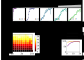
\includegraphics[width=0.7\textwidth]{figures/4_primacy_coding_SI}
\caption{Additional results pertaining to the primacy coding hypothesis. 
\textbf{A} Percent of active ORNs required for 75\% accuracy of a steep sigmoidal odor step, as a function of odor step intensity and odor complexity. For low complexities, a primacy set of fewer ORNs may be sufficient to decode the full odor signal; for higher complexities, the entire ORN repertoire is required.
\textbf{B} In the primacy coding hypothesis, the primacy set is realized sooner for stronger odor signals, so odors are decoded earlier in time, resulting in a perceptual time shift with increasing odor concentration ~\cite{primacy_coding}. We also find this shift in our compressed sensing decoding framework (right plot), which rises monotonically with step height for various odor complexities, in agreement with primacy coding.
\textbf{C} The consistency of a primacy code across changes in background odor concentration, in a system with Weber Law adaptation. We calculate the primacy set for odor A (step odor; black) in the presence of either a weak, medium, or strong background (dotted lines; 1x, 10x, 100x a.u.), assuming the system has adapted its response to the background as described in the main text. Averaged across odor A identities, primacy sets for odor A when in the 1x background are nearly identical to those when odor A is in the 10x background (right plot; yellow). The same holds true when comparing the 1x and 100x backgrounds, for sufficiently large primacy order, above 8 or so right plot; purple). This indicates that Weber Law adaptation preserves primacy codes across disparate environmental conditions.
}
\label{fig:SI_primacy}
\end{figure}



\renewcommand\thefigure{\ref{fig:downstream}--figure supplement 1}  



\begin{figure}
    \centering
    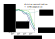
\includegraphics[width=0.6\textwidth]{figures/5_downstream_SI.pdf}
    \caption{Accuracy of binary classification  by odor valence, for odors whose concentrations span a narrow range of concentrations (1 order of magnitude). Accuracy is plotted as a function of the number of distinct odor identities classified by the trained network, in systems with only ORN adaptation, only divisive normalization, both or neither. Decoding gains conferred by divisive normalization and/or ORN adaptation are much smaller than when odors span a much larger range of concentrations, as shown in the main text.}
    \label{fig:SI_downstream}
\end{figure}

\end{document}